\section*{Question 1}
\emph{Investigate the stability and accuracy of the four schemes in terms of the Courant-Friedrichs-Lewy (CFL) numbers $\lambda = c \tfrac{dt}{dx}$ and $\mu = \nu \tfrac{dt}{{dx}^2}$. In particular use numerical experimentation and/or von Neumann stability analysis to determine stability boundaries.}



The stability boundary is probed numerically by varying dt, since the convection and diffusion are fixed. Changing $\Delta x$ is also unnecessary since $k = \sigma/c = 0.05$ and in consequence $k \Delta x \approx 3.6\times 10^{-4} \ll 2\pi$. The code in Listing \ref{code1} was used to probe the stability boundary numerically for increasing $\Delta t$. The criteria for changing the truth flag is stored in the 

\lstinputlisting[label=code1, language=Octave, caption=Code used to find the maximum time step and the resulting CFL parameters]{probe.m}

\begin{table}[ht!]
\caption{CFL coefficients and time step for a stable boundary}
\label{tbl1}
\centering
\begin{tabular}{l|c|c|c}
& Convection $\lambda$ & Diffusion $\mu$  & $dt$\\ \hline
Euler - Central Diff 2 & $2.753e-03$ & $3.758e-06$ & $2.0162e-05$\\
Euler - Central Diff 4 & $2.731e-03$ & $3.729e-06$ & $2.0002e-05$\\
RK2 - Central Diff 2 & $2.731e-02$ & $ 3.728e-05$ & $2.000e-04$ \\
RK2 - Central Diff 4 & $1.365e-01$ & $1.864e-04$ & $1.000e-03$\\
\end{tabular}
\end{table}


%
%\begin{figure}[!ht]
%\centering
%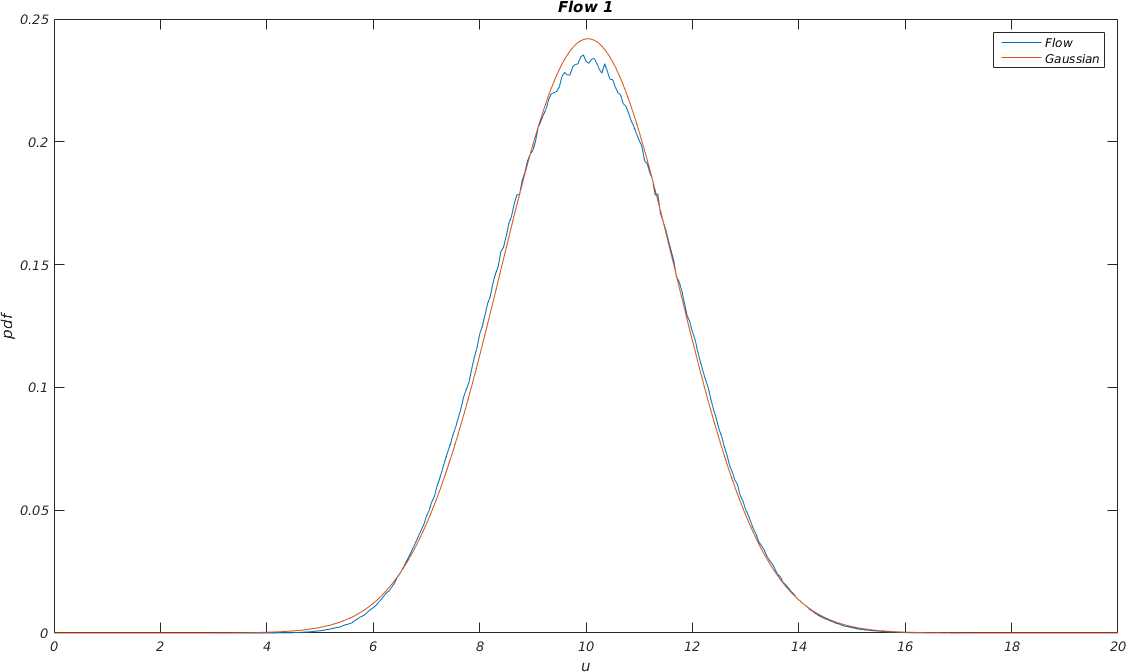
\includegraphics[scale=0.4]{./TEXT/pdf1.png}
%\caption{The Probability Density function for \emph{flow 1}}
%\label{pdf1}
%\end{figure}
%
%
%\begin{table}[ht]
%\caption{Comparison of the first four moments for the two flows.}
%\label{tbl1}
%\centering
%\begin{tabular}{l|c|c}
%& Flow 1 & Flow 2 \\
%\hline
%1\su{st} Moment: Mean & $10.04$ & $10.04$ \\
%\hline
%2\su{nd} Moment:Variance & $2.72$ & $2.72$ \\
%\hline
%3\su{rd} Moment:Skewness & $0.05$ & $0.05$\\
%\hline
%4\su{th} Moment:Kurtosis & $2.78$ & $2.78$ \\
%\hline
%\end{tabular}
%\end{table}
%
